\chapter{Discussion}\label{chapter:discussion}

One aim of the master thesis was to investigate whether GraphQL can bring performance improvement in micro-frontend architectures. The improvement should be accomplished by using a single caching layer for all micro-frontends and a mechanism to reduce queries by utilizing the cache. The technology agnosticism prototypical implementation is also discussed in this chapter. The results of evaluating the caching improvements of the prototypical micro-frontend implementation architecture are also discussed in this chapter. The results from Chapter \ref{chapter:results} are used to make a statement about the hypothesis from Chapter \ref{chapter:introduction}. The next sections focus on discussing the results in terms of request size and response size. 

\section{Request Size}

This section compares the different measurements of the request sizes. Figure \ref{fig:discussion:request-size} displays the results from the previous chapter \ref{section:results:comparison-first-journey} and \ref{section:results:comparison-second-journey} as a bar chart for better comparison. As shown in the figure the difference in request size is not very significant. The two approaches with the shared cache do not save network request resources. The difference between the first 

11 requests omitted
The reduction of queries only makes 1.64 KB difference, in contrast to only sharing the cache.

\begin{figure}[H]
  \centering
  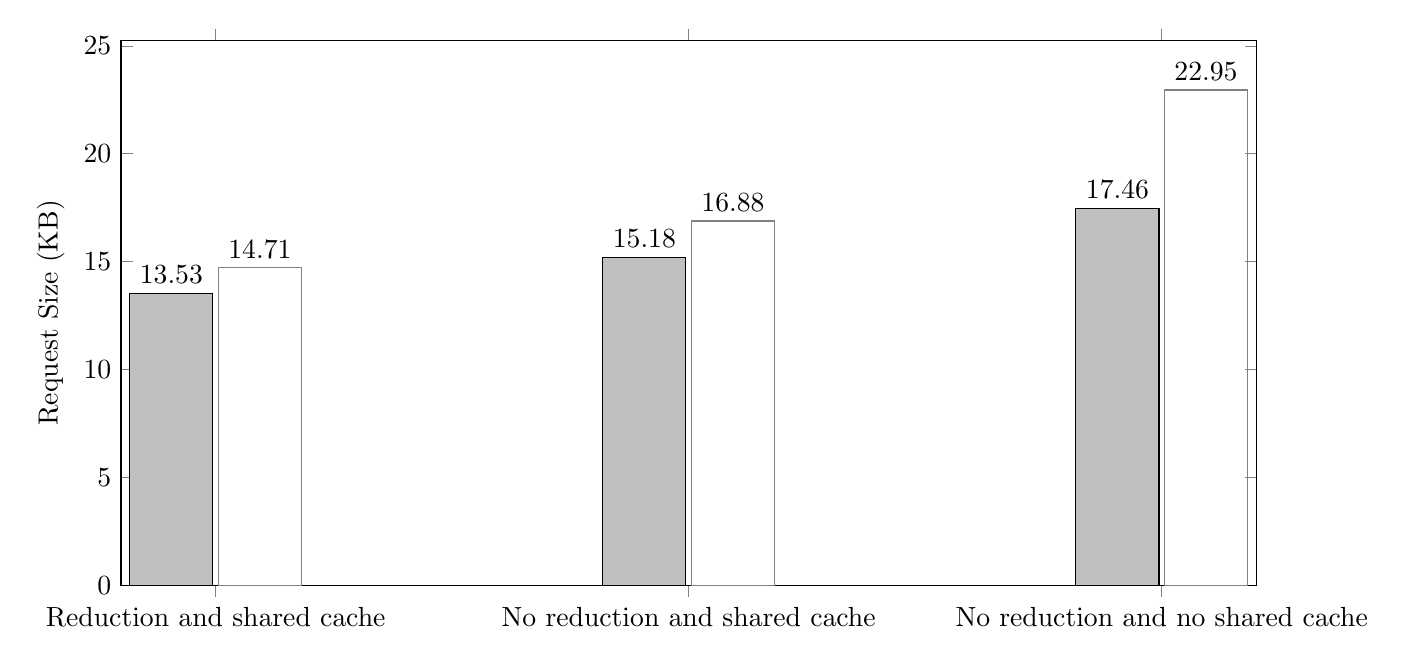
\begin{tikzpicture}
    \begin{axis}[
      ymin=0,
      ybar,
      ylabel={Request Size (KB)},
      xtick=data, 
      symbolic x coords={Reduction and shared cache, No reduction and shared cache, No reduction and no shared cache}, 
      nodes near coords align={vertical},
      nodes near coords,
      height=8.5cm,
      width=16cm,
      bar width=30pt,
      cycle list={
        {fill=lightgray, draw=gray}
      },
    ]
    \addplot coordinates {(Reduction and shared cache, 13.53) (No reduction and shared cache, 15.18) (No reduction and no shared cache, 17.46)};
    \addplot coordinates {(Reduction and shared cache, 14.71) (No reduction and shared cache, 16.88) (No reduction and no shared cache, 22.95)};
    \end{axis}
  \end{tikzpicture}
  \caption{Request size comparison of the three approaches.}\label{fig:discussion:request-size}
\end{figure}

\section{Response Size}

Figure \ref{fig:discussion:response-size} displays the results already shown in the previous chapter as a bar chart. In contrast to the request size, the response sizes are very far apart. When comparing the naive approach with the two improved approaches, there is a difference of about 2.40 MB. However, when comparing the two improved approaches, the difference is not very large. For the records that the application fetches, the reduction does not make such a big difference, in terms of responses. 

\begin{figure}[H]
  \centering
  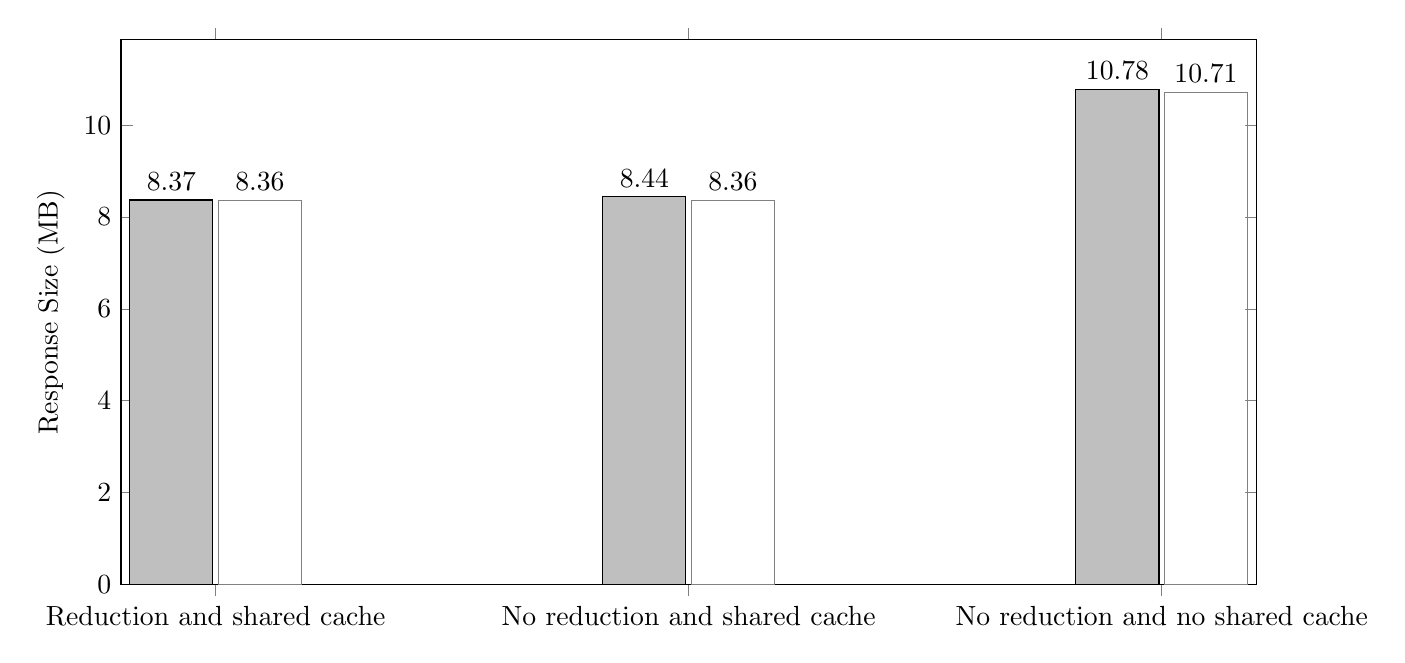
\begin{tikzpicture}
    \begin{axis}[
      ymin=0,
      ybar,
      ylabel={Response Size (MB)},
      xtick=data, 
      symbolic x coords={Reduction and shared cache, No reduction and shared cache, No reduction and no shared cache}, 
      nodes near coords align={vertical},
      nodes near coords,
      height=8.5cm,
      width=16cm,
      bar width=30pt,
      cycle list={
        {fill=lightgray, draw=gray}
      },
    ]
    \addplot coordinates {(Reduction and shared cache, 8.37) (No reduction and shared cache, 8.44) (No reduction and no shared cache, 10.78)};
    \addplot coordinates {(Reduction and shared cache, 8.361) (No reduction and shared cache, 8.364) (No reduction and no shared cache, 10.71)};
    \end{axis}
  \end{tikzpicture}
  \caption{Response size comparison of the three approaches.}\label{fig:discussion:response-size}
\end{figure}
